\chapter{Accommodation in Multiparty Interaction with An Agent}
\label{chap:speech_variations_in_hhci}

\lettrine{M}{ore} dynamic vocal behaviors can be established in interaction with more than two speakers.
This is not only due to additional possible connections between interlocutors, but also because of additional factors that might influence them as well, like the order of speech or the role of each speaker.
A \acl{hhci} study is presented in this chapter, where the effects of different aspects and conditions on vocal accommodation are investigated.

\pagebreak

\section{Speech variations in human-human-computer interaction}
\label{sec:accommodation_in_multiparty_interaction_with_an_agent}

Nowadays, we are witnessing in our everyday lives an ever-growing presence of devices with spoken interaction capabilities, like \acp{pa}, speech-activated cars, hands-free medical assistants, and \acp{its}, to name a few.
As argued in \cref{subsec:personal_assistants}, the use of \acp{pa} is rapidly increasing, as more every-day tasks can be achieved using them.
The question arises, therefore, whether different speech patterns and characteristics emerge in such \ac{hci} than in \ac{hhi}; and if yes, which.
One way of measuring such changes is in terms of linguistic similarity between the interlocutors.
It has been demonstrated that humans may change their speech behavior when interacting with computer-based systems.
In various \ac{hci} experiments, participants have been shown to speak differently to computers in general, and also change their speech during the interaction (see \citet{Branigan2010linguistic}, for examples).
The vast majority of experimental work done in the field of vocal accommodation deals with the smallest possible social interactions, namely dyadic conversations.
Those can be dyads of two human speakers, forming \ac{hhi}, or a human and some computer-based agent, which results in \ac{hci}.
Vocal accommodation in these types of interactions is explored in \cref{chap:shadowing_in_sung_music_and_human_computer_interaction,chap:conv_analysis}.
However, social interactions may also be multiparty, consisting of three or more participants.
this is true for both \ac{hhi} and \ac{hci}, but also for interactions with mixed human and computer-based interlocutors.
The last can occur in various situations, like a person consulting a \ac{va} regarding availability in a weekly schedule while setting an appointment with a colleague or two friends ordering tickets from a voice-activated machine.
Such mixed multiparty interactions already take place in our every-day lives.
Their popularity -- and sometimes necessity -- increase alongside the rise in use of \ac{c-ai} devices, such as \acp{va}, voice-activated cars, social robots, etc.
It is important, therefore, to investigate whether convergence, divergence, and other effects (see \cref{subsec:variation_types}) can be found not only in \aclp{hci}, but in \acp{hhci} as well.
Various \ac{hci} experiments have shown that participants speak differently to computers in general, and also change their speech behavior during the interaction, e.g., by \citet{Branigan2010linguistic} and \citet{Levitan2016implementing}.
And yet, no previous work in the field performed a direct comparison between different human-directed and computer-directed speech couplings within a multiparty interaction.
If any direct comparison is done in empirical \ac{hci} experiments, it typically focuses on computer-based interlocutors only and emphasizes the influences of different system configurations on the interaction \citep[e.g.,][]{Levitan2016implementing}.
Moreover, only the influence of the system's speech output on the user speech is examined, but not the influence of other human interlocutors.

Empirical work on multiparty \ac{hci} includes experiment where participants interact with different types of agents, like social robots \citep[as in][]{Foster2012two,Ibrahim2019fundamental} and human avatars in immersive virtual worlds \citep[e.g.,][]{Traum2002embodied}.
Even in dyadic form, spoken interactions are a hard task for computers.
All the more so, when more than one other interlocutors are involved.
Measuring accommodation becomes more complex with multiple interlocutors involved, as discussed in \citet{Rahimi2019acoustic}.
There are many technical challenges on the way to realistic, real-time interactions with computers, including -- but not limited to -- center-of-attention detection, active speaker detection, turn taking, understanding private and shared knowledge, and of course correct speech production and understanding.
Interactions with machines are challenging for humans, too, since the former do not behave and react the same way (and usually speed) as humans.
An example of such a social activity, which is easy for humans to learn but still far from being accomplished by social robots, along with ways to cope with it, are described in \citet{Jonel2018Farmi}.
The type and severity of those problems depend also on the type of computer-based agent.
For instance, embodied agents at least have some basic way to convey non-verbal information, whereas voice-only systems like \acp{va} do not.
On the one hand, this gives a wider range of expressions to embodied systems, but requires more communication channels to implement on the other hand.
See \cref{sec:types_of_sdss} for more information about the different types of computer-based agents.

This chapter presents a study that examines interaction-level vocal accommodation in a \acf{hhci} scenario, focusing on distributional and temporal analyses of three phonetic features (see \cref{sec:analysis_hhci})
In this paradigm, two human speakers interact with an agent to complete tasks with a common goal.
More details about the dataset and the tasks are in \cref{sec:vacc}.
Investigating such a scenario contributes to the understanding of both the role of an agent in interactions with multiple humans and the role of one human interlocutor on the other.
These two aspects are examined in the two \emph{components} of the study:
The \emph{addressee} component focuses on the differences between the participants' addressed interlocutor within a conversation \citep[][see]{Raveh2019ESSV}, and the \emph{crowd} component spotlights the influence of an additional human interlocutor on the participants' speech toward the agent \citep[see][]{Raveh2019InterspeechAlexa}.
The question tackled by the second component is whether and to what extent speaking to a second human interlocutor in addition to Alexa influences the accommodation in interaction with a \ac{va}.
More generally, it investigates whether users speak differently towards a computer-based system when another human participates in the interactions.
The performed analyses in \cref{sec:analysis_hhci} are based on the participants' \emph{speech directions}, i.e., \acf{hds} and \acf{dds}, as illustrated in \cref{fig:condition_comparison_addressee,fig:condition_comparison_crowd}.
The comparisons were made based on the tasks performed by participants using the \ac{va} in both components, alternately interacting with the \ac{va} alone or with a confederate.
\todo{need more motivation for the two components?}

\section[The voice assistant conversation corpus]{Dataset} % \acl{vacc} doesn't work for some reason
\label{sec:vacc}

The \acf{vacc}\footnote{\url{http://www.iikt.ovgu.de/iesk/en/Research+Groups/MDS/Research/VACC-p-4624.html}}, introduced in \citet{Siegert2018VACC}, was utilized to examine these differences.
This corpus is suitable as it comprises both \acp{hci} and \acp{hhci} (\emph{solo} and \emph{confederate} conditions) with a 2\textsuperscript{nd} generation Amazon Echo Dot device with the skills and a female voice of the \acf{va} Alexa.
Other studies, like \citet{Shriberg2013addressee,vanTurnhout2005identifying}, used similar corpora to study automatic addressee detection.
The present work does not set detection and classification as a goal, but rather aims to provide insights and measures that might be useful for such tasks.
In the \ac{vacc}, the confederate was only present in the room only during tasks in the confederate condition and always sat at the same location.
To simulate the spatial situation of a multi-party interaction with a \ac{va}, the participant and the male confederate sat in similar distance from the device that was situated on a table, roughly forming an equilateral triangle shape in a living room-like environment (see Figure 2 in \citet{Siegert2018VACC}).
The participant had led the interactions, and the confederate never initiated the interaction.
Moreover, the confederate interacted only with the participant and never with Alexa.

%Two high-quality neckband microphones (Sennheiser HSP 2-EW-3) were used to capture the voices of the participant and the confederate speaker.
%Additionally a high-quality shotgun microphone (Sennheiser ME 66) captured the overall acoustics and the output of Amazon's Alexa.

In both conditions, two interactions took place, one for each task of the performed tasks:
The participant's goal in the calendar task is to find available time slots for several appointments with the confederate.
The participant's pre-defined calendar is stored on the device and is accessible only by inquiring Alexa.
In the solo condition, the participants got written information about the confederate's availability, whereas, in the confederate condition, the confederate could be asked directly about it, resulting in \acp{hhi} along side the \acp{hci}.
\cref{fig:conditions_comparison} illustrates the relations in each condition.
The goal of the quiz task is to answer trivia questions, e.g., \enquote{When was Albert Einstein born?}
Since Alexa was not always able to immediately provide a full answer to all the questions, the required information could be gathered incrementally in multiple steps.
Here, the participant solved the quiz alone in the solo condition or teamed up with the confederate so the two could discuss the question-asking strategy in the confederate conditions.
The quiz task is generally less formal than the calendar task.
%
\begin{figure}[t]
	\centering
	\subfigure[Solo condition]
	{\raisebox{1.85cm}{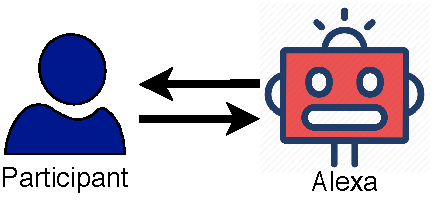
\includegraphics[width=0.45\textwidth]{condition_solo}}
	\label{fig:condition_solo}}
	\hfill
	\subfigure[Confederate condition]
	{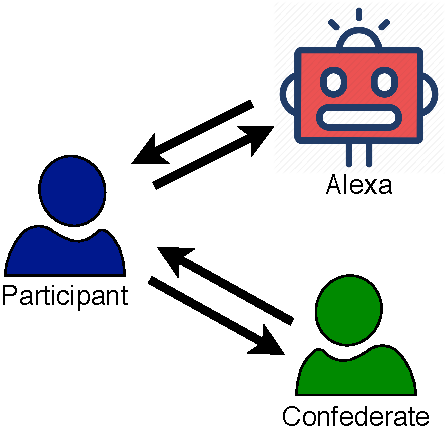
\includegraphics[width=0.45\textwidth]{condition_confederate}
	\label{fig:condition_confederate}}
	\caption[Solo and confederate conditions in \acs{hhci} setting]
		{Illustration of solo and confederate conditions.
		A black arrow represents direction of speech from speaker to addressee.
		Note that the confederate (in green) never talks or addressed by Alexa, but only the participant (blue).}
	\label{fig:conditions_comparison}
\end{figure}
%
The calendar task is designed so that the way to its solution is relatively straightforward:
Query the device for possible times till a match is found.
This requires interacting mostly -- if not only -- with the computer-based interlocutor.
Indeed, this task typically elicited interactions, in which the participant interacted with the confederate or the device in discretely separate turn blocks in the confederate conditions.
\ac{dds} blocks were, unsurprisingly, longer, as the confederate was only needed when additional information about the task was required.
The way to solve the quiz task is more flexible, because the strategy as to which questions to ask Alexa can be determined by the participant, including the amount and frequency of the confederate's intervention in the confederate conditions.
Indeed, this led to a more dynamic alteration between \ac{hds} and \ac{dds} in this task.

The dataset contains recordings of 27 (14 female) German native speakers in the age range of 20 to 32 years (mean 24~$\pm$3.3).
Each participant performed the quiz and calendar tasks in both solo and confederate conditions, for a total of 108 interactions (2 tasks $\times$ 2 conditions $\times$ 27 participants).
%An interaction was finished either by completing the task or by stopping it prematurely in case no further progress could be made, to avoid participant frustration.
%The latter, however, happened only a few times.
These interactions consist of approximately \num{13500} utterances, which were manually transcribed and annotated (speaker, speech times, addressee, etc.) and stretch over total recording time of \SI{17}{\hour} \SI{7}{\minute} (\SI{31}{\minute} average interaction length).
The permutations of the tasks, conditions, and their order were balanced.

%\begin{figure}[!h]
%	\begin{center}
%		\fbox{\parbox{6cm}{
%		This is a figure with a caption.}}
%		\includegraphics[scale=0.5]{image1.eps} 
%		\includegraphics[width=0.75\linewidth]{figures/IMG_4798.jpg}
%		\caption{A snapshot of the data collection setup. The confederate speaker (left side) and the participant (right side) are sitting around a table, where the voice assistant (Amazon Alexa Echo Dot) is located.}
%		\label{fig:wohnzimmer}
%	\end{center}
%\end{figure}


%The recordings were stored in WAV format with \SI{44.1}{\kilo\hertz} sample rate and 16 bit resolution.
%The recordings were manually separated into utterances, which were additionally annotated with its speaker, context, and textual transcription.
%The speaker of each utterance could be the participant, Alexa, or the confederate.
%The context marked the type of interaction of the utterance, which include \ac{hds}, \ac{dds}, cross-talk, off-talk, laughter, and more.
%To deal with clearer data, only \ac{hds} and \ac{dds} contexts were used for analysis in this paper.
%The transcription was obtained using the Google Cloud Speech API automatic speech recognition service.
%\cref{tab:dataset_charact} summarizes the dataset characteristics.

%\begin{table}[t]
%	% \captionsetup{format=plain,justification=raggedleft,width=.4\textwidth,hangindent=0pt,skip=500pt}
%	\centering
%	\caption{\ac{vacc} dataset characteristics}
%	\label{tab:dataset_charact}
%	\begin{tabular}{L{3cm}L{3cm}}
%		\toprule
%	     Participants 				& 27														\\
%	     Sex 						& Male 13 / Female 14 										\\
%	     Total Recorded Data 		& \SI{17}{\hour} \SI{7}{\minute}							\\
%	     Experiment Duration 		& Mean: 31 min 												\\
%		  Age (years)				& Mean 24 (Std: 3.32)										\\	% Min: 20; Max: 32  \\
%	     Language 					& German													\\
%	     Annotation 				& Transcription, Addressee, Laughter, Cross-Talk, Off-Talk	\\ 
%	     Supplementary self-reports & Evaluation of interaction, AttrakDiff, Speaking style, Experiences in interacting with voice assistants\\
%		\bottomrule
%	\end{tabular}
%\end{table}

\begin{figure}[t]
	\centering
	\subfigure[\acs{hds} in confederate condition]
	{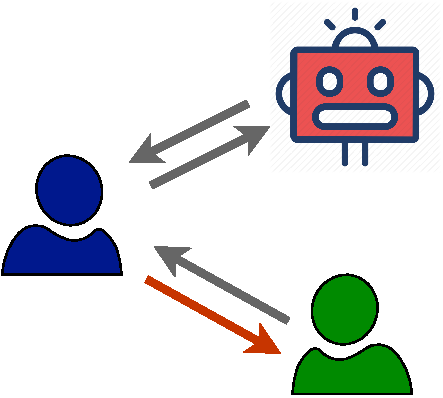
\includegraphics[width=0.45\textwidth]{condition_confederate_marked_hhi}
	\label{fig:condition_confederate_marked_hhi}}
	\hfill
	\subfigure[\acs{dds} in confederate condition]
	{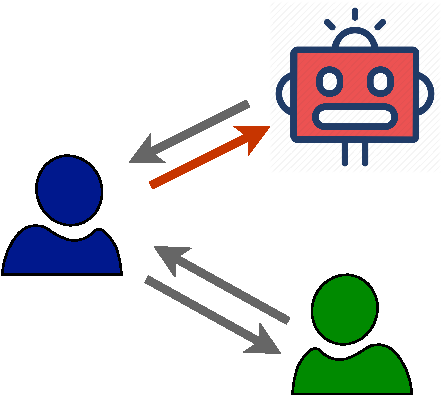
\includegraphics[width=0.45\textwidth]{condition_confederate_marked_hci}
	\label{fig:condition_confederate_marked_hci}}
	\caption[\acs{hds} and \acs{dds} compared in confederate condition]
		{Illustration of the compared speech directions in the \emph{addressee component}.
		The orange arrows mark the compared speech directions.}
	\label{fig:condition_comparison_addressee}
\end{figure}

\begin{figure}[t]
	\centering
	\subfigure[\acs{dds} in solo condition]
	{\raisebox{1.6cm}{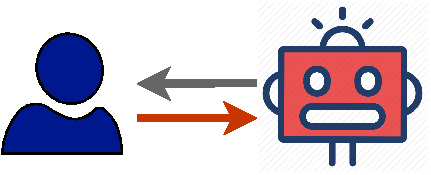
\includegraphics[width=0.45\textwidth]{condition_solo_marked}}
	\label{fig:condition_solo_marked}}
	\hfill
	\subfigure[\acs{dds} in confederate condition]
	{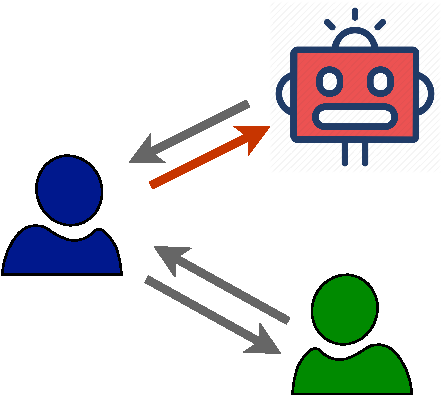
\includegraphics[width=0.45\textwidth]{condition_confederate_marked_hci}
	\label{fig:condition_confederate_marked_hci_crowd}}
	\caption[\acs{dds} compared in solo and confederate conditions]
		{Illustration of the compared speech directions in the \emph{crowd component}.
		The orange arrows mark the compared speech directions.}
	\label{fig:condition_comparison_crowd}
\end{figure}

\subsection{Annotations}
\label{subsec:annotations_hhci}

Each utterance in an interaction was annotated with its speaker, context, and textual transcription.
The speaker of each utterance could be the participant, Alexa, or the confederate.
Cross-talk was rare, as the participants typically waited till the confederate or Alexa finished talking (exception occurred when they tried to interrupt Alexa mid-utterance when the response was undoubtedly wrong or irrelevant due to recognition error).
The context marks the utterance's interaction type, like \ac{hds}, \ac{dds}, cross-talk, off-talk, laughter, and more.
To deal with clearer data, only \ac{hds} and \ac{dds} contexts were used for analysis, which, together, constitute over \SI{90}{\percent} of the overall recording time.
The transcriptions were obtained using the Google Cloud Speech API automatic speech recognition service and were subsequently manually verified and corrected.
Utterances' start and end times were directly derived from the timestamps of these annotations.

\section{Analysis}
\label{sec:analysis_hhci}

A suitable subset of the entire dataset (see \cref{sec:vacc}) was used for the analysis of each factor (see \cref{sec:accommodation_in_multiparty_interaction_with_an_agent}).
Only the 54 interactions from the confederate conditions were used for the addressee component, as the alternation between \ac{hds} and \ac{dds} within an interaction was examined.
For the crowd component, all 108 interactions were taken, because the comparison required executions of the tasks performed in both solo and confederate conditions.
Interactions of all 27 participants were included in both subsets.
Despite the different sizes of the subsets, the number of comparisons was the same for both factors, since the addressee component used two both speech directions of the participants in each interaction (54 $\times$ 2 = 108) and the crowd component used only one speech direction but from both conditions (54 $\times$ 1 + 54 $\times$ 1 = 108).
These subsets were analyzed based on the audio signals and the annotations described in \cref{subsec:annotations_hhci}.
The speaker annotations were used to determine to which of the three speakers the measured values should be ascribed.
The text transcriptions were only used to verify the correct audio segments were analyzed.
Comparisons were made between the speech directions in the same interaction, i.e., within a single task.

To increase temporal resolution, the audio signals were cut into two-seconds \emph{slices}.
A single slice always contained audio from a turn of a single speaker.
Any remainder shorter than \si{2} seconds got a slice of its own.
For example, a turn of \SI{5.2}{\second} in length was sliced into three slices of \SI{2}{\second}, \SI{2}{\second}, and \SI{1.2}{\second}.
This way, each slice contained speech of a single interlocutor.
Splitting the turn also creates equal, consecutive, and more comparable time units for an interaction without introducing artificial boundaries by dividing it into a pre-defined number of parts \citep[as in][]{Silber-Varod2018prosodic}.
This is especially important for the temporal analysis (\cref{subsec:temporal_analysis}).
Slice lengths of 0.5, 1, 5, and 10 seconds were experimented with as well.
However, those were found too short to capture changes in \ac{ar}, which is dependent on the size of this window, or two long to for a comparable and uniform temporal resolution.
Two seconds was found to be a good compromise based on these criteria.
%
The following phonetic features were targeted: 
%
\begin{description}%[wide=0pt, leftmargin=0.5\parindent, nosep]
	\item[\Acf{f0}] -- mean pitch measured within a slice with hop size of \SI{100}{\milli\second} and a defined range between \SIlist{60;350}{\hertz}.
	\citet{Gregory1993Voice} found that this feature is used to produce social similitude and cohesiveness in dyadic interviews.
	\citet{Babel2012role} found convergence effects in this feature in an auditory naming task and \citet{Bulatov2009effect} found similar effects in a shadowing task.
	
	\item[Intensity] -- mean intensity measured within a slice with hop size of \SI{100}{\milli\second}.
	This feature showed significant entrainment effect in game scenarios in \ac{hhi} experiments described in \citet{Levitan2011measuring}.
	Accommodation effects in this feature were also found by \citet{Natale1975convergence}.
	
	\item[\Acf{ar}] -- the ratio of the number of syllables to phonation time within a slice, as described in \citet{DeJong2009arcitulcationrate}.
	\citet{Schweitzer2013convergence} examined this feature in the context of phonetic convergence, but no effect was found on turn-level and interaction-level analyses.
\end{description}
%
All features were measured individually in each slice automatically using Praat \citep{Boersma2018praat} scripts.

\section{Results}
\label{sec:results_hhci}

Two analyses were carried out: distributional and temporal.
The first looks at global differences on the interaction level of the participant's and the computer-based interlocutor's productions between solo and confederate conditions.
It also examines whether the order in which the tasks were performed had any influence on the changes (see \cref{tab:signif_conditions,fig:signif_cases_ordered}).
The second examines time-based, continuous changes in the proximity between the participant's and the device's productions with an emphasis on the context factor (\ac{dds} or \ac{hds}), and provides additional insights for the factors \emph{sex}, \emph{task}, and \emph{order} (\cref{fig:condition_convergence_comparison,fig:alluvial}).

\subsection{Distributional analysis}
\label{subsec:distributional_analysis}

As a first measure of speech characteristics, the means, medians, and \aclp{sd} of the selected features in the participants' speech in each of the interactions were calculated in \ac{hds} and \ac{dds}.
The absolute values reflected in the means and medians can shed light on the overall range of values used with each of the two interlocutors, due to, for example, their gender (Alexa was always set with a female voice and the confederate was always male) or assumed comprehension capabilities of humans and computers.
The variability in the \aclp{sd} reflects of each interlocutor may indicate a different production behavior.
\todo[inline]{is it meaningful to have a table with these lists/values?}
Each target feature was measured and listed chronologically throughout the interaction.
These lists were divided into four distributions based on speaker and context:
the participant talking to the confederate, the participant talking to Alexa, the confederate talking to the participant, and Alexa talking to the participant (cf.\ four speech directions in \cref{fig:condition_confederate}).
The contrast between \ac{hds} and \ac{dds} is observable within the participant's speech only, which was active in both contexts.
The significance level of the difference between these two distributions was measured using a two-sample t-test with $\alpha=0.05$.

\Cref{fig:hds_dds_dist_signif,fig:hds_dds_dist_nonsignif} show examples of the distributions of a participant's \ac{f0} in \ac{hds} and \ac{dds} contexts.
Since Alexa always used a female voice and the confederate was always male, there is a natural gap between their \ac{f0}.
This gap leaves room for convergence to occur, i.e., change in the participants' production -- either temporarily or fixedly -- in the direction one of the other interlocutors.
As \cref{tab:results_hhci_addressee} shows, in \SI{74}{\percent} of the cases out of the 54 analyzed interactions the difference of the participant's \ac{f0} between \ac{hds} and \ac{dds} was significant.
Out of those, in \SI{85}{\percent} of the cases \ac{dds}'s distribution mass contained higher values than \ac{hds}'s, which indicates assimilation towards Alexa.
%
\begin{figure}[t]
	\centering
	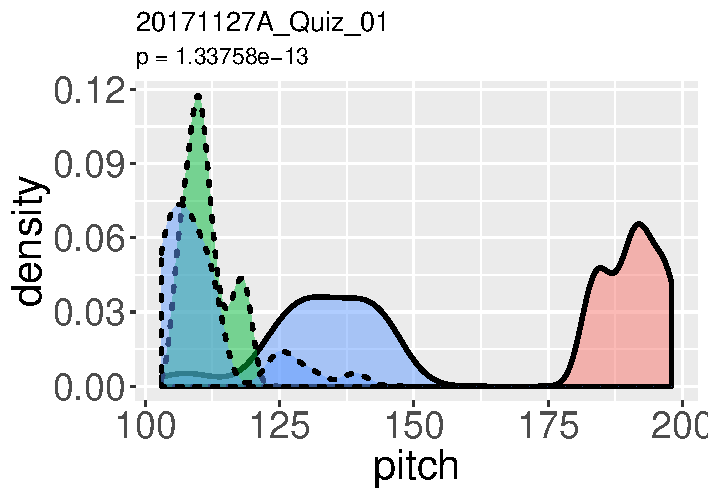
\includegraphics[width=\linewidth]{20171127A_Quiz_01_pitch_dist}
	\caption[An interaction with significant \acs{hds} and \acs{dds} \acs{f0} distributions difference]
		{An example of \ac{hds} and \ac{dds} distributions with a \emph{significant} difference (p-value~$\ll$~0.0001 with $\alpha=0.05$) extracted from the \ac{f0} measures in the quiz task of participant 20171127A.
		The colors represent distributions of Alexa (red), the confederate (green), and the participant (blue).
		The line style differentiates between \ac{hds} context (dashed line) and \ac{dds} context (solid line).}
	\label{fig:hds_dds_dist_signif}
	\todo[inline]{change p value notation in figure to <<}
\end{figure}
%
\begin{figure}
	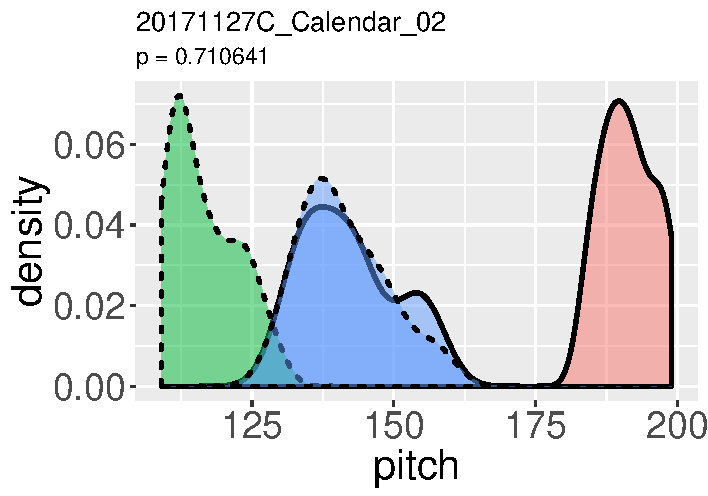
\includegraphics[width=\linewidth]{20171127C_Calendar_02_pitch_dist}
	\caption[An interaction with insignificant \acs{hds} and \acs{dds} \acs{f0} distributions difference]
		{An example of \ac{hds} and \ac{dds} distributions with a \emph{insignificant} difference (p-value~=~0.71 with $\alpha=0.05$) extracted from the \ac{f0} measures of participant 20171127C in the calendar task.
		The colors represent distributions of Alexa (red), the confederate (green), and the participant (blue).
		The line style differentiates between \ac{hds} context (dashed line) and \ac{dds} context (solid line).}
	\label{fig:hds_dds_dist_nonsignif}
	\todo[inline]{change p value notation in figure to <<}
\end{figure}
%
%\cref{fig:hds_dds_violin_intensity_comparison} shows examples of the distributions of the participant's intensity in \ac{hds} and \ac{dds} contexts.
Unlike in the case of \ac{f0}, absolute measured values of intensity may not be as meaningful due to the device's and the confederate's location relative to the participant's microphone, was used for the different analyses
This means that the absolute values of the participant's intensity in \ac{hds} and \ac{dds} can be compared directly, but only indirectly with Alexa's and the confederate's.
Therefore, the differences in \cref{fig:hds_dds_dist_signif,fig:hds_dds_dist_nonsignif} can be compared within a context, but the values should only be compared within the participant's speech (in blue).
In \SI{89}{\percent} of the cases the difference of the participant's intensity between \ac{hds} and \ac{dds} was significant.
Generally speaking, participants tended to speak to Alexa with a louder voice than to the confederate.
%
\begin{figure}[t]
	\centering
	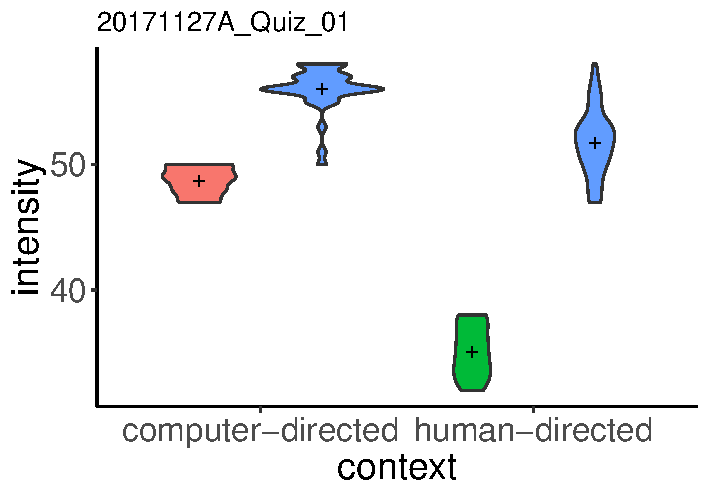
\includegraphics[width=\linewidth]{20171127A_Quiz_01_intensity_violin}
	\caption[An interaction with significant \acs{hds} and \acs{dds} intensity distributions difference]
		{An example of \ac{hds} and \ac{dds} distributions with a \emph{significant} difference (p-value~$\ll$~0.0001, $\alpha=0.05$) extracted from the intensity measures of participant 20171127A in the quiz task.
		A non-significant example is presented in \cref{fig:hds_dds_violin_nonsignif}.
		The colors represent distributions of Alexa (red), the confederate (green), and the participant (blue).
		The width of the box represents the frequency of the values and the \enquote*{+} sign marks their respective means.}
	\label{fig:hds_dds_violin_signif}
	\todo[inline]{legend and units for y-axis}
	\todo[inline]{explain in text that comparison is only relative between two blue components}
\end{figure}
%
\begin{figure}
	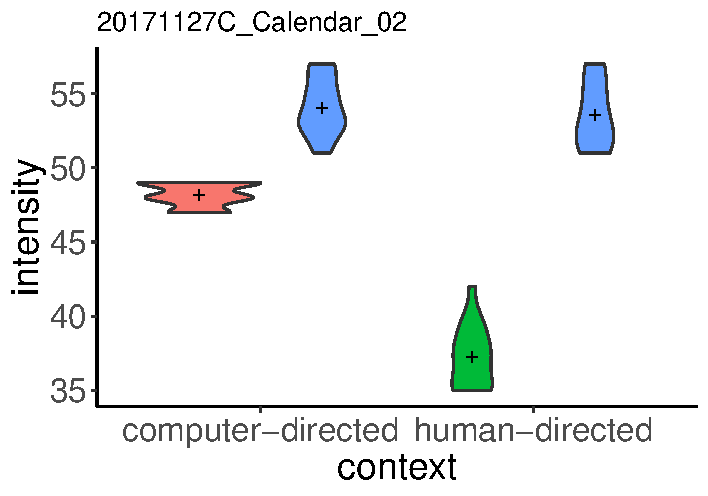
\includegraphics[width=\linewidth]{20171127C_Calendar_02_intensity_violin}
	\caption[An interaction with insignificant \acs{hds} and \acs{dds} intensity distributions difference]
		{An example of \ac{hds} and \ac{dds} distributions with a \emph{insignificant} difference (p-value~=~0.55, $\alpha=0.05$) extracted from the intensity measures of participant 20171127C in the calendar task.
		A significant example is presented in \cref{fig:hds_dds_violin_signif}.
		The colors represent distributions of Alexa (red), the confederate (green), and the participant (blue).
		The width of the box represents the frequency of the values and the \enquote*{+} sign marks their respective means.}
	\label{fig:hds_dds_violin_nonsignif}
	\todo[inline]{legend and units for y-axis}
	\todo[inline]{explain in text that comparison is only relative between two blue components}
\end{figure}
%
The differences between \ac{ar} distributions in \ac{hds} and \ac{dds} were calculated as well.
In \SI{13}{\percent} of the cases out of the 54 analyzed interactions the difference of means of the participant's \ac{hds} and \ac{dds} \ac{ar} distributions was significant.
This shows that the participants largely spoke with the confederate at the same speed as the device.
It was found that the articulation rate was lower in some specific cases where the participant tried to improve intelligibility, specifically when the system's output indicated that it could not understand the participant's previous utterance.
%While such utterance-level changes are interesting and may point to a temporary change in behavior, a more detailed analysis is outside the scope of this study, which concentrates on interaction-level behavior.
%
\begin{table}[t]
	\centering
	\caption[Percentage of significantly different interaction pairs in addressee component]
	{Percentage of interaction pairs with significant differences with respect to each target feature with all the interactions together and separated by order tasks.}
	\label{tab:signif_conditions}
	\sisetup{table-format=3.0}
	\begin{tabularx}{\linewidth}{XSSS}
		\toprule
		\thead[l]{feature} & {\thead{any order}} & {\thead{solo first}}	& {\thead{confederate first}}\\
		\midrule
		\acs{f0}	& 67	& 72	& 60 \\
		intensity 	& 67	& 76	& 56 \\
		\acs{ar}	& 30	& 31	& 28 \\
		\bottomrule	
	\end{tabularx}
\end{table}
%
\begin{figure}[t]
	\centering
	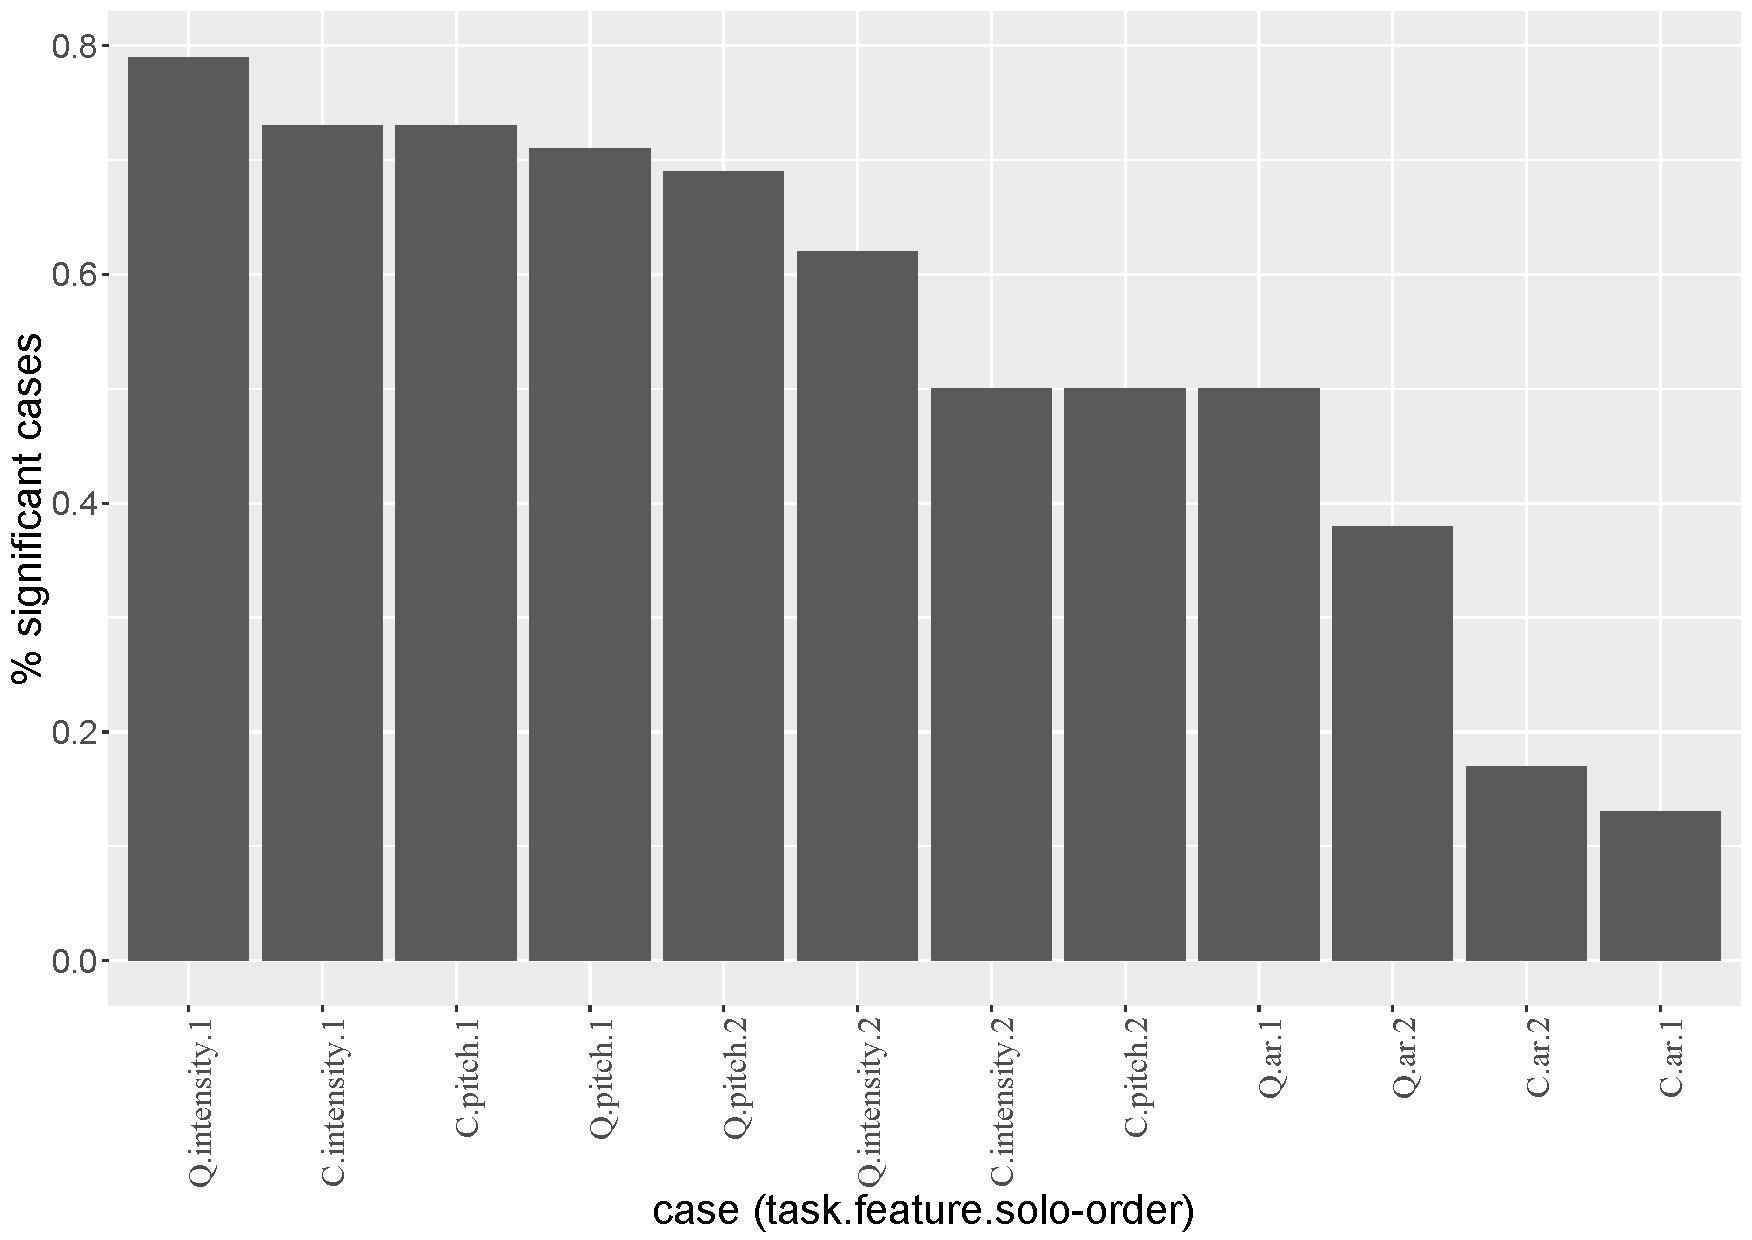
\includegraphics[width=\linewidth]{barplot_signif_cases}
	\caption[Per-case comparison of significant distributional differences in the crowd component]
		{Percentage of instances with a significant difference between solo and confederate conditions in each case.
		A case is a combination of the factors \emph{task}, \emph{feature}, and \emph{order}.
		For example, the case \emph{Q.intensity.2} contains the comparisons of intensity in interactions of the quiz task where solo condition was performed second (and the confederate condition first).}
	\label{fig:signif_cases_ordered}
\end{figure}
%
\begin{figure*}[t]
	\centering
	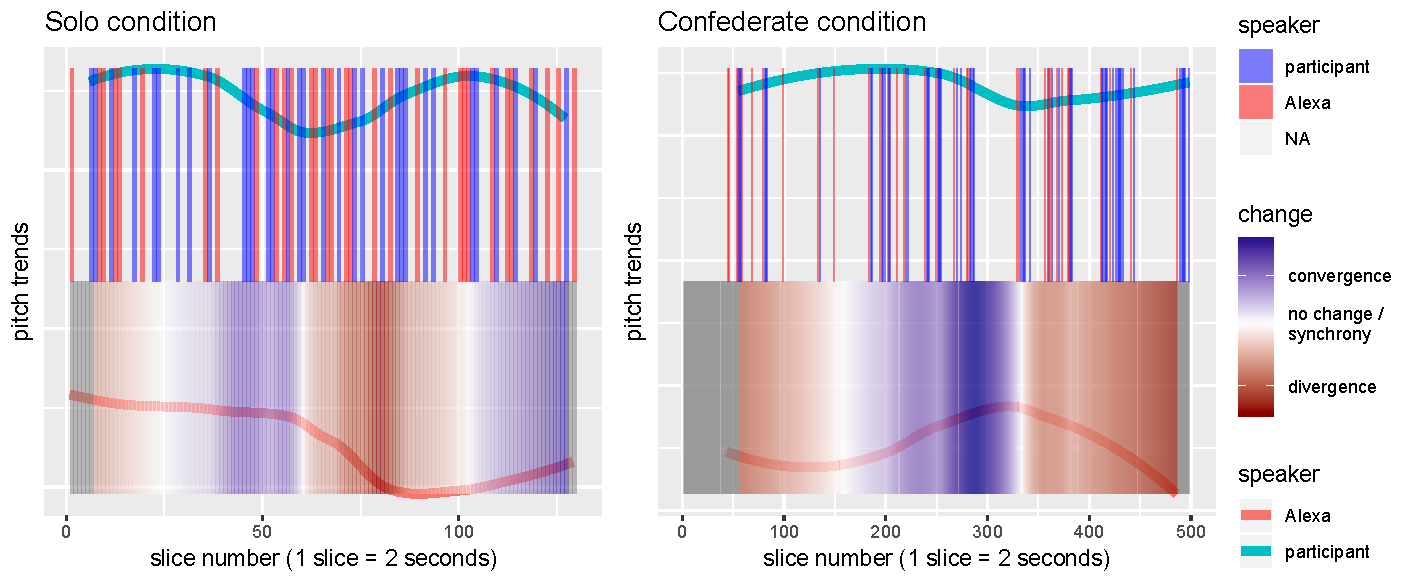
\includegraphics[width=\linewidth]{20171127B_Quiz_pitch}
	\caption[Temporal comparison of accommodation in solo and confederate conditions]
		{A comparison between the behavior of the \ac{f0} feature in solo condition (left) and confederate condition (right).
		The lines represent the \ac{loess} smoothing trend lines of the participant (blue) and Alexa (red).
		Omitted turns, e.g., turns of the confederate and turned removed as explained in \cref{sec:method} are not colored (gray).
		The vertical bars in the upper half represent the turns of the participant (blue) and Alexa (red).
		The color-scaled vertical bars at the bottom half are the convergence/divergence level of the participant over time as calculated in \cref{eq:accommodation}.
		Blue areas represent convergence while red areas represent divergence.
		The darker the color, the greater the effect, with white color pointing to points of no change (or synchrony, in segments with both trends moving the same way).}
	\label{fig:condition_convergence_comparison}
\end{figure*}
%

The distributional analysis examines the differences between the participant and Alexa's speech in solo and confederate conditions in terms of the general behavior of the participants with respect to the target features.
This general behavior is determined by the set of values of the target features produced by the participants in each condition.
Since this analysis checks whether the participants behave differently as a whole towards the non-human speaker, the temporal order of the values is not considered.
To detect these differences, the distribution of their respective values in the solo and confederate conditions in each interaction pair were compared.
This was done by using the two-sample Wilcoxon test \citep{Wilcoxon1945individual}, with $\alpha = 0.05$ with the null hypothesis that similar distributions of the target feature were used in both conditions.
A significant result of the test means that the participant produced the respective feature differently when interacting with Alexa alone compared to when the confederate participated as well.
\cref{tab:signif_conditions} shows the percentage of interaction pairs, in which the null hypothesis was rejected, i.e., that the feature was utilized differently by the participant in each condition.
Since chronologically, by design, one of the conditions needed to precede the other, the percentages were also calculated separately for the cases where tasks were performed first in the solo condition (and then in the confederate condition), and vice versa.
This separation shows whether interacting first with Alexa alone, without any human input, influenced the vocal behavior of the participants.
As there were no breaks between the interactions, the only factors for change were the order of the conditions and the involvement of another human speaker.
Indeed, the percentages of significant differences when interacting first only with Alexa were higher by \SI{12}{\percent}, \SI{20}{\percent}, and \SI{3}{\percent} for \ac{f0}, intensity, and \ac{ar}, respectively.
\cref{fig:signif_cases_ordered} further breaks down the differences between interaction pairs and introduces the factor of the performed task.
In line with the tendency shown in \cref{tab:signif_conditions}, the features \ac{f0} and intensity have the highest percentages of significant cases, regardless of the performed task, and the tasks performed first show higher percentages of different distributions.
In the lower percentages, it is the task, rather than the target feature, that shows differences between the cases.
And last, for \ac{ar}, with the lowest percentages, there is a clear difference between the quiz and the calendar tasks.
All in all, the \emph{task} factor was a good indicator only for the feature with the lowest difference percentage and the \emph{order} factor was more informative for the features with higher percentages.
To sum up, these results show significant differences in the majority of the cases for two of the three features for both the addressee and crowd components.
These outcomes provide a look into further aspects of \ac{hds} and \ac{dds} and speech-related features in conversation analysis, which may help studies in topics like addressee detection or  multiparty \ac{hci}.

\subsection{Temporal analysis}
\label{subsec:temporal_analysis}

Looking at the distribution differences of the selected features in \ac{hds} and \ac{dds} sheds light on the general speech behavior tendencies.
However, this analysis leaves out an important aspect of spoken interactions, namely the time dimension.
While the interaction-level distributions measures show the overall range and frequency of the values, temporal analysis adds the information as to how they changed over time.
Adding the time dimension gives an overview of the interaction's structure and reveals fine-grained information regarding its characteristics, such as turn lengths, turn switching, pauses, the density of a speaker's utterances, accommodation effects, and more.
For example, \cref{fig:hds_dds_time_pitch} shows a case where the absolute \ac{f0} values are roughly the same in \ac{hds} and \ac{dds}, around \SI{150}{\hertz}, but the behavior of the participant is different.
In the \ac{dds} context, the participant generally keeps a stable distance from Alexa's voice, whereas in the \ac{hds} context the \ac{f0} values are closer to the confederate.
In both contexts, the participant's \ac{f0} starts around \SI{150}{\hertz}, but in \ac{hds} the minimum \ac{f0} is only slightly below this initial value, whereas in \ac{dds} it drops as far as \SI{25}{\hertz} lower.
A similar example of the intensity feature is shown in \cref{fig:hds_dds_time_intensity}.
Unlike the previous example, here the absolute values steadily differ by about \SI{5}{\decibel}, but the overall change is similar.
That is, in both cases the intensity rises from the beginning to around a quarter of the interaction's duration, and then decreases again until the end (in \ac{hds} more quickly than in \ac{dds}) down to approximately the same value as at the beginning.

Since \cref{fig:hds_dds_time_comparisons} shows two examples of the quiz task performed by two different participants, it is possible to compare the structure of these interactions as well.
As described in \cref{sec:vacc}, the quiz task in the confederate condition is designed so that the two human speakers need to find an effective way to solve the questions using Alexa.
After improving their strategy, the lead should ultimately be taken by the participant, who interacts with Alexa to solve the questions as quickly and correctly as possible.
In both examples, the interaction starts with relatively short turns and rapid context changes.
This might be ascribed to the fact that the participant is still trying to figure out the best way to interact with Alexa and the confederate.
Then, sometime after the middle of the interaction, there is a larger block of \ac{dds}, followed by some more turns of \ac{hds}, possibly discusses with the confederate about ways to solve the last questions.
Finally, the interactions end with a shorter block of \ac{dds}, in which the participants finish these last questions of the quiz.
This structure was found to be the typical flow of the quiz task across participants.
%
\begin{figure}[t]
	\centering
	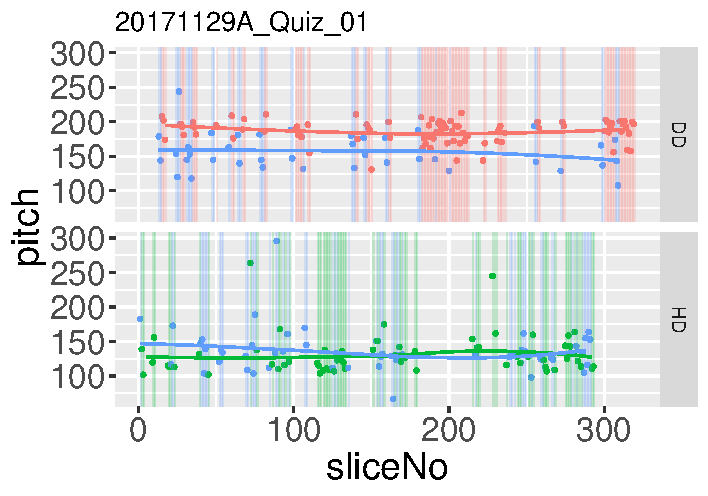
\includegraphics[width=\linewidth]{20171129A_Quiz_01_pitch_time}
	\caption[Comparison of temporal \acs{f0} trends of \acs{hds} and \acs{dds}]
		{The changes of intensity over time in \ac{dds} (upper part) and \ac{hds} (lower part).
		The timespans on the x-axis are represented by turn slices, as explained in \cref{sec:analysis_hhci}, and the y-axis shows the value of the feature.
		A slice's background color indicates the speaker in this slice and the circle with the same color, the measured value of the feature in it.
		Alexa's voice is shown in red, the confederate in green, and the participant in blue.
		The lines are smoothed values calculated by LOESS \citep{Cleveland1988locally}.
		In \ac{dds}, the speaker starts a bit above \SI{150}{\hertz} and ends slightly beneath it, generally maintaining the distance from the device's values.
		In \ac{hds}, the contour starts around the same value as in \ac{dds}, but gradually goes down towards the confederate and then up again, staying in the same range of values as the human speaker.
		This shows a different behavior with similar values.}
	\label{fig:hds_dds_time_pitch}
\end{figure}
%
\begin{figure}[t]
	\centering
	{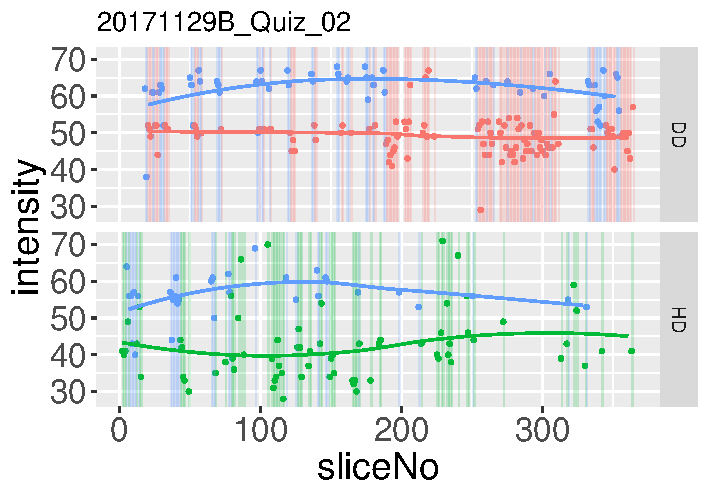
\includegraphics[width=\linewidth]{20171129B_Quiz_02_intensity_time}
	\label{fig:hds_dds_time_intensity}}
	\caption[Comparison of temporal intensity trends of \acs{hds} and \acs{dds}]
		{The changes of intensity over time in \ac{dds} (upper part) and \ac{hds} (lower part).
		The timespans on the x-axis are represented by turn slices, as explained in \cref{sec:analysis_hhci}, and the y-axis shows the value of the feature.
		A slice's background color indicates the speaker in this slice and the circle with the same color, the measured value of the feature in it.
		Alexa's voice is shown in red, the confederate in green, and the participant in blue.
		The lines are smoothed values calculated by LOESS \citep{Cleveland1988locally}.}
		In both \ac{hds} and \ac{dds} contexts, there are a rise and a fall around the same time in the participant's values.
		However, the absolute values differ.
		This shows a similar overall behavior with different values.
	\label{fig:hds_dds_time_comparisons}
\end{figure}
%
\begin{table}[t]
	\centering
	\caption[Percentage of significantly different interaction pairs in crowd component]
		{Summary of results. The percentage of interactions in which the difference of distribution means was significant for each feature, and their mean and \acf{sd}.}
	\label{tab:results_hhci_addressee}
	\begin{tabularx}{\linewidth}{XSSS}
		\toprule
		& \acs{f0} 						& {intensity}				& \acs{ar}									\\
		signif. diff.					& \SI{74}{\percent}			& \SI{89}{\percent}		& \SI{13}{\percent} \\
		\acs{hds} mean (\acs{sd}) 		& 10.5\,\si{\hertz}			& 2.95\,\si{\decibel}	& 0.627				\\
		\acs{dds} mean (\acs{sd}) 		& 10 \,\si{\hertz}		& 2.61\,\si{\decibel}	& 0.634				\\
		\bottomrule	
	\end{tabularx}
\end{table}
%	
Another way to look at accommodation in an interaction is in the temporal dimension.
In this analysis, the same raw measured values were used to examine changes that occur over time.
That is, unlike the analysis presented in \cref{subsec:distributional_analysis}, here the order of the values (i.e., their change over time) plays a major role, and effects may be found in specific time windows.
To perform such an analysis over the entire interaction, two additional computation steps are required.
First, each point in time must have a corresponding value for each feature produced by all speakers.
This was achieved by smoothing the measured value using \ac{loess} \citep{Cleveland1988locally}, a non-parametric regression method that deterministically fits a function to a localized subset of the data.
The fitting was done for each speaker separately over all slices of \ac{hds}/\ac{dds} with measured values of the features.
This results in a predicted value for each slice of the conversation.
\cref{fig:condition_convergence_comparison} shows an example of these smoothed measures of one participant and Alexa for the \ac{f0} feature.
The lower part of the figure shows the accommodation changes of the participant during the interaction (blue for convergence and red for divergence), and the upper part shows the turn-taking events.
The confederate condition has fewer turn events, as the analysis concentrates on the participant and Alexa, and the confederate turns are not shown.
Secondly, the relationship between a feature's values in each slice needs to be determined to describe their temporal changes.
Since we are interested in accommodative behavior, a measure for the relative change between slices was used.
It calculates the participant's contribution to the overall change in proximity between the participant and Alexa.
Alexa's contribution is considered to be a static effect, as it is not directly changing based on the user's speech input, and is therefore not taken into account.
The change tendency between two slices is calculated by
%
\begin{equation}
	\label{eq:change}
	change_t = -\Delta_{t, t-1} \mid S_{part} - S_{Alexa} \mid,
\end{equation}
\eqname{Smoothed change tendency of two interlocutors}\noindent
%
where the index $t$ refers to the current slice and $S_{part}$ and $S_{Alexa}$ are the smoothed values of the participant and Alexa, respectively.
The minus sign at the front flips the value so that increased proximity (convergence) is represented by positive values and distancing (divergence) by negative values (see \cref{fig:condition_convergence_comparison}).
Subsequently, the participant's contribution toward the accommodation is calculated by
%
\begin{equation}
	\label{eq:accommodation}
	accomm(participant)_t = change_t - \Delta_{t, t-1} S_{Alexa}.
\end{equation}
\eqname{Speaker's own contribution to mutual accommodation}\noindent
%
The sum of the proximity changes of each target produced by all participants in every sex-task-condition-order combination was calculated, resulting in a single value that represents the overall change.
A value greater than zero means that more convergence was observed, and a negative value points to more divergence.
There were only two instances where this value was exactly zero, both for the \ac{ar} feature.
These instances were treated as cases of divergence, for their divergence spans were longer.
Using this approach, only a few interactions had no feature convergence in them, and several had all three features showing convergence.
However, a stricter approach was applied, where a feature was considered as converging only if its overall accommodation value was higher than one standard deviation from its mean.
Based on that, all interactions were categorized by the number of features that showed more convergence in them.
\Cref{fig:alluvial} summarizes the categorization for each factor individually.
Each line represents a single interaction.
The strata labels through which each line passes, indicate the group it belongs to with respect to each factor.
The number of features that showed more convergence than divergence overall is marked by the color of the line.
Some tendencies emerge from this categorization:
first, in \SI{35}{\percent} of the interactions, there was at least one feature that showed convergence, but in none of them did all three features do so.
In seven interactions, two features showed convergence, twice by males and five times by females.
In total, males converged in \SI{5}{\percent} of all measurements and females in \SI{7}{\percent}.
Furthermore, of all the instances of converged features, \SI{58}{\percent} occurred in the solo condition, compared to \SI{42}{\percent} in the confederate condition.
However, no difference between the calendar and quiz tasks was found, with \SI{49}{\percent} and \SI{51}{\percent} of the cases, respectively.
The same holds for the comparison between the two orders in which the tasks could be performed.
These results support the addition of the confederate to the interaction as the factor for less convergence.
%
\begin{figure}[t]
	\centering
	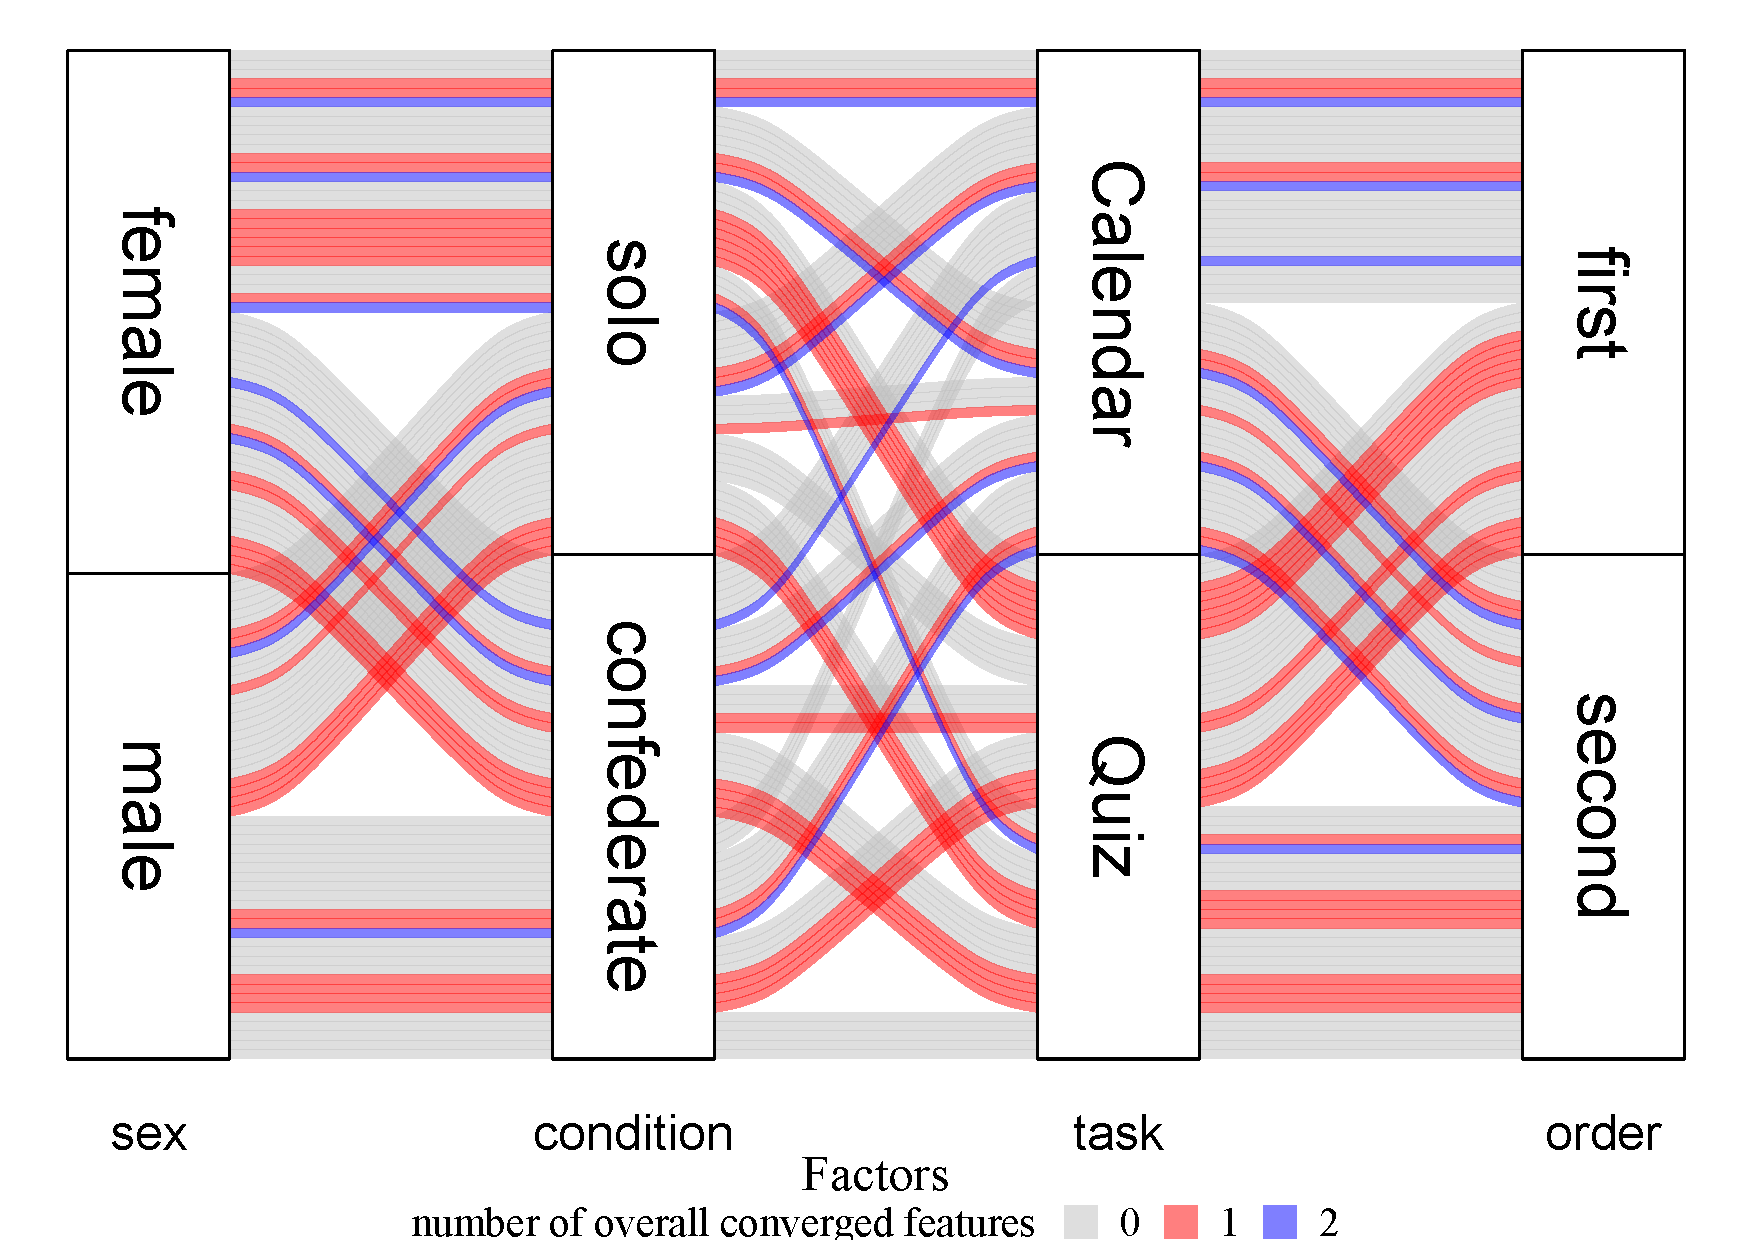
\includegraphics[width=\linewidth]{alluvial_4factors_numConv_strict}
	\caption[Number of significantly different behaviors per factor]
		{Overview of the relation between the factors \emph{sex}, \emph{condition}, \emph{task}, and \emph{order} and the number of features that showed more convergence in total across the interactions.
		Each line represents one interaction.
		The \emph{sex} stratus refers to the sex of the participant, and the \emph{order} stratus to the position of an interaction in the order in which the task-condition combination was performed.
		The color of a line stands for the number of target features that showed overall convergence in this interaction, from none (zero features, in gray), through one (red), and up to two (blue).
		%		and up to all three features (green).
		For example, a blue line going through the strata sequence female $\rightarrow$ solo $\rightarrow$ quiz $\rightarrow$ first represents an interaction with a female participant performing the quiz task in solo condition first, where the participant converged in two out of the three target features.}
	\label{fig:alluvial}
\end{figure}
%
\section{Conclusion}
\label{sec:discussion_hhci}

\emph{Addressee} and \emph{crowd} components examined different aspects of a simulated real-world use case, in which a human user talks alternately with a computer-based interlocutor and another human interlocutor.
\cref{sec:accommodation_in_multiparty_interaction_with_an_agent} introduces this modern-day means of communication and where it occurs.
Distributional and temporal accommodation analyses were performed for these components to provide interaction-level and time-sensitive insights.
Results for the three target vocal features, \ac{f0}, intensity, and \ac{ar}, are presented in \cref{sec:results_hhci}.

On the component level, the first two features show a greater degree of difference in both components, and the latter, a smaller one.
Furthermore the changes are even larger in the crowd component, in which a human interlocutor is involved, than in the addressee component.
This indicates that \ac{f0} and intensity are generally more prone to variation than \ac{ar}, and hints that human interlocutors trigger these variations more.
There might be two reasons for this difference.
First, computer-based agents, including Amazon Alexa, do not change their speech output in any way, regardless of the user's input and variation in it.
As a social, dynamic, mutual process, accommodation is more likely to be stronger if both interlocutors contribute to the overall effect.
In this experiment, the process can only be mutual in \ac{hds}, where accommodation may occur naturally (cf.\ \cref{sec:communication_accommodation_theory}).
Secondly, due to this natural, spontaneous nature of accommodation in \ac{hhi}, the participants probably automatically spoke differently, more dynamically, in \ac{hds}, since the expectation for similar variation and dynamics is inherently expected from a human interlocutor.
Finally, \acp{va} (and voice-activated devices as a whole) are, in most cases, still not performing well enough for people to speak to them as fluently and dynamically as with other humans.
This has technical reasons, but the result is a different consciousness while talking to machines.
For example, users are more likely to articulate whole sentences, typically without reformulating, when requested to repeat their utterance by the device, whereas human interlocutors are capable of requesting and conveying corrections for shorter segments of utterances using intonation and other means.
Furthermore, although generally more seldom vary, users tend to reduce their \ac{ar} when repeating their utterances to the device, or when trying to be more clear.
This resembles the way people talk to children when they want to be more clear.
However, due to the way \ac{asr} systems are trained, more often than not this achieves the opposite result.
This reduced speaking rate phenomenon is discussed further below.

Regarding the individual features, one possible explanation for the different \ac{f0} distributions is the natural difference in male and female \ac{f0} (Alexa used a female voice while the confederate was always male), which leaves room for accommodation for participants of both sexes.
In that case, the results shown here point to the fact that the participants generally treated Alexa as a human interlocutor with regards to \ac{f0} behavior, as opposed to, for example, matching only the human interlocutor and talking to the computer-based interlocutor using the same, somewhat monotonous \ac{f0}.
A similar effect was found for intensity.
Since the device and the confederate were spaced approximately at the same distance from the participants, there was no apparent reason for the participants to speak more loudly with either interlocutor.
Therefore, an explanation of the tendency to speak more loudly to the device may come from the intuition that a computer-based system has a harder time understanding human speech and therefore needs a clearer signal.
This stands in line with the interpretation presented above that humans sometimes treat voice-activated devices as humans who need a hyper-articulated signal, e.g., toddlers or language learners\footnote{In a sense, this analogy is correct, as the devices -- or rather their \ac{asr} components -- indeed learn to process speech signals.
Despite that, this process is not identical to the way babies learn this, and therefore such projection on the speech style does not help the device improving its understanding of the user.
The technical and psychological differences and consequences of that are beyond the scope of this chapter.}.
Another explanation may be the illusion that Alexa feels more distant than the human interlocutor because she is not an embodied agent \citep[cf.][and see \cref{sec:types_of_sdss} for further details]{Staum2010virtually, Gijssels2016speech}.
Keeping in mind that an interaction aims to be as efficient as possible using minimum effort, it seems like changing these features helped the participants -- or at least felt like they did -- to interact more efficiently with the device.
Regardless of whether this roots from the unconscious attempt to treat the device like a human interlocutor or the fact that accommodation occurs, even if to a lesser extent, even when not mutual, the effect still takes place.
This is, however, not the case with \ac{ar}, which shows a lower percentage of significant differences.
This indicates that \ac{ar} does not tend to vary as much as \ac{f0} and intensity, which stands in line with other studies, like \citet{Schweitzer2013convergence}.
Slower, more carefully articulated speech, occurs less often in regular speech than louder speech or higher pitch.
Such enhanced articulation not only takes longer to produce, but also requires more effort, making it a less preferred way to communicate, unless necessary.
In this somewhat formal, experimental setting, participants are likely to speak more slowly than usual, and the motivation to complete the task in a short time does not encourage them to speak even more slowly.
This supports the hypothesis that extra slow speech would only be used when necessary, e.g., when a repetition is required due to a misunderstanding of an utterance, as discussed above.
Even in that case, the overall \ac{ar} tends to increase afterwards, to make the interaction more fluent again.
These local, short-term variations may suggest that changes in \ac{ar} are done more consciously than in other phonetic features.

The results presented in \cref{tab:results_hhci_addressee,tab:signif_conditions} show that for all three features
\begin{enumerate*}[(a)]
	\item the distributions differed more when the participants first interacted with the device alone, and
	\item more convergence was aggregated in the task that was performed first.
\end{enumerate*}
Furthermore, the factors \emph{sex} and \emph{task} indicated that female participants showed less convergence than male participants, but the task performed did not play any role in increasing the amount of convergence.
The first speech input a participant encounters may cause a priming effect that, together with the natural tendency to converge to an interlocutor, results in a greater change in interactions that occur first.
However, the interchangeability of input (here, both \ac{hhi} and \ac{hci}) seems to hinder the ability of the participants to converge to Alexa.
One explanation for this may be that it is more natural for humans to accommodate to other humans, so once another human is involved, the accommodation towards the computer interlocutor is neglected.
Another possible explanation is that due to the multiple interlocutors, the participants do not have a steady target towards which to accommodate, which leads to a weakened convergence effect.
This is confirmed by the higher rate of convergence in the solo condition compared to the confederate condition.
Since \ac{hci} still lacks the mutuality of a comprehensive accommodation effect, the question arises whether these tendencies would be stronger in interactions with a single human versus interactions with two different human speakers simultaneously.
The higher number of convergence instances by female participants may be ascribed to the \ac{va} using a voice of the same sex and could be further investigated by using a \ac{va} with a male voice.
Temporal analysis showed higher degrees of alignment towards Alexa in the solo condition.
This could be explained as a reaction to a more stable vocal target (especially since Alexa generally doesn't change her voice much) than when speaking to two entities alternately.
From the collaborative point of view, this may also be due to the fact that the participants wanted to create better collaboration relations to improve effectiveness.
This is a natural, even automatic, process that occurs in \ac{hhi}, but of course does not affect, as for today, computer-based interlocutors.
In general it was clear that accommodative effects and tendencies were present in both conditions, which is reassuring for future multiparty \ac{hci} accommodation research.
Two main open questions remain concerning the temporal aspect of interactions.
The first has do to with analysis on the speech \emph{signal level}, where the changes in measures over time can capture phenomena like convergence or divergence.
In a more comprehensive analysis in this direction, more detailed patterns may emerge.
Such an analysis can concentrate on one context or on comparing patterns in both \ac{hds} and \ac{dds}.
Additionally, more features can be measured to reveal more details regarding speech behavior.
The second may highlight behavioral patterns of the conversation on the \emph{turn levels}.
This can include a closer examination of the interaction structure as a whole, the dynamics of turn changes, pauses and repetitions, etc.
Such an analysis can be performed on interactions in solo and confederate condition to inspect whether humans deal with the same task performed with a computer alone differently than when another human is involved.